\section{Results and discussion}

In this section we detail the findings of our study. We present the results of the first and
second studies in Section~\ref{sec:res-fs} and Section~\ref{sec:res-ss}, respectively. In Section~\ref{sec:discussion} we summarize the
implications of our study. 

\subsection{Result of the first study: A \blls replication}\label{sec:res-fs}

Our first study is a replication of the \blls.
As discussed in the previous section, we first executed the analysis using the DroidXP benchmark with its default
configuration. Then we repeated the process, however this time we isolate the effect of the static analysis component of DroidFax. In this way, we could better estimate the performance of the dynamic analysis tools for mining Android sandboxes.
Table~\ref{tab:fs} summarizes the results of the executions. The columns Exec. (WS) and Exec. (WOS) 
show the number of malwares identified when executing each tool with the
support of the DroidFax static analysis algorithms (WS) and without the support
of DroidFax static analysis algorithms (WOS). 
The Impact column shows 
(in percentage) to what extent the DroidFax static analysis algorithms influences
the performance of the sandboxes created after
executing the test generation tools. We calculate the impact
using Eq. (1).

\begin{eqnarray}
Impact & = & \frac{(Exec.\ (WS) - \ Exec.\ (WOS)) \times 100}{Exec.\ (WS)} 
\end{eqnarray}  


Table~\ref{tab:fs} shows that the impact of DroidFax in the results is significant, ranging
from 16.44\% (DroidBot) to 51.79\% (Humanoid). Note that, in the \blls, the authors do not present a
discussion about the influence of DroidFax in the performance of the
test generation tools, even though this influence is not negligible. 
Considering the \joke
tool, our fake test generation tool that does not execute the apps during
the benchmark execution, DroidFax improves the performance in 100\%.
This result is expected, since the \joke tool does not execute any dynamic analysis.
Next we discuss the result of each individual test generation tool. 

\begin{table}[ht]
  \caption{Summary of the results of the first study. }
  \centering
  \begin{small}
 \begin{tabular}{lrrr}
   \toprule
   Tool & Exec. (WS) & Exec. (WOS) & Impact (\%) \\   \midrule
   DroidBot &  73 & 61 & 16.44 \\ 
   Monkey &  71 & 56 & 21.13 \\ 
   DroidMate &  68 & 52 & 23.53 \\ 
   Humanoid &  56 & 27 & 51.79 \\ 
\joke &  42 & 0 & 100.00 \\ 
 \bottomrule
 \end{tabular}
 \end{small}
 \label{tab:fs}
\end{table}

\begin{description}
\item[DroidBot] in the first execution (Exec. WS) led to a sandbox that detected a total of $73$ malware among $96$ pairs present in our dataset ($76.04$\%),
  detecting more apps with malicious behavior than any other tool. Similar to the \blls, DroidBot is the test case generation tool
  whose resulting sandbox detected the largest number of malicious apps. Moreover, in our second execution (Exec. (WOS)), removing the DroidFax
  static analysis support reduced the DroidBot performance in 16.44\%, the smaller impact we observed among the tools.

  \item[Monkey] in the first execution (Exec. (WS)) produced a sandbox that detected $71$ out of the $96$ pairs of Android apps.
    Contrasting, in the original study, the Monkey's sandbox detected $48$ malwares within the 102 pairs ($47.05$\%). This difference
    might be due to the fact that Monkey uses a random strategy for test case generation and here we considered the outcomes
    of three executions---while in the \blls, the authors consider the outcomes of one execution. 
    Considering our second execution (Exec. (WOS)), there is a reduction of $21.13$\% in the Monkey's performance, leading to
    a sandbox that was able to detect $56$ malwares. 

  \item[DroidMate] in the first execution (Exec. (WS)) led to a sandbox that detected 68 apps with malicious behavior ($70.83$\%).
    In the \blls study, DroidMate also detected $68$ malwares, though considering the $102$ pairs of apps used in the
    original study. In the second execution (Exec. (WOS)),
    without the DroidFax static analysis algorithms, the resulting sandbox's performance drops by $23.53$\%, being able to detect
    52 out of the 96 pairs of Android apps.
    
  \item[Humanoid] showed the worst performance, even though a previous work~\cite{DBLP:conf/kbse/LiY0C19} presented that it leads to
    the highest number of lines coverage in comparison to Monkey, DroidBot, and DroidMate. This might suggest that test generation
    tools that try to simulate the human behavior, such as Humanoid, are less effective to build Android sand boxes, in comparison
    with techniques that rely on random testing (such as Monkey). In the first execution (Exec. (WS)),
    the resulting Humanoid sandbox identified $56$ malwares in our dataset ($58.33$\%). Humanoid was the most affected in the second
    execution (Exec. (WOS)), whose resulting sandbox presents a reduction of $51.79$\%  in the number of detected malwares.
    Since the \blls did not explore Humanoid,
    we do not have a baseline for comparison with the previous work.

  \item[\joke] is our fake test case generation tool that help us understand the performance of the DroidFax static analysis algorithm for mining sandboxes. 
  %\kn{joke seems to be defined here but used before}
    We integrated \joke into the DroidXP benchmark as an additional test case generation tool that does not run the Android apps.
    As a result, the analysis using \joke reveals the performance of DroidFax static analysis algorithms alone. For the first execution, with the DroidFax static
    algorithms enabled, even though \joke does not execute the Android apps, its resulting sandbox detected 43.75\% of the malwares. For the second execution,
    that is, disabling the DroidFax static analysis algorithm, the resulting \joke sandbox was not able to detect any malware. Therefore,
    our results show that DroidFax alone is able to detect more than 40\% of the malicious version of the apps. 

\end{description}


\begin{finding}
  Integrating the dynamic analysis tools
  with the DroidFax static analysis algorithms
  improves substantially the performance
  of the resulting Android sandboxes for
  detecting malicious behavior. 
\end{finding}
 
The Venn-diagram of Figure~\ref{fig:venn-plot1}
summarizes how the tools can complement each other.
Note in the diagram that $53$ malwares have been detected
by all sandboxes generated in the first execution (with the DroidFax static analysis algorithms),
out of the 78 malwares identified by at least one sandbox. In addition, the DroidMate sandbox did not detect
any malware that had not been detected by the other tools. Differently, the Monkey sandbox detected
three malwares that had not been detected by any other sandbox, the DroidBot sandbox detected two malwares
that had not been detected by any other sandbox, and the Humanoid sandbox detected one malware that had not
been detected by any other sandbox. 
Contrasting with the \blls,
our results suggest that using DroidMate in combination with Monkey, DroidBot, and Humanoid
does not improve the general performance of an integrated environment for mining
Android sandboxes.

\begin{finding}
  Our results suggest that one might benefit from using  an integrated
  environment that combines Monkey, DroidMate, and Humanoid to
  mine Android sandboxes. Introducing the DroidMate 
  tool does not improve the results.
\end{finding}


\begin{figure}[htb]
  \centering{
  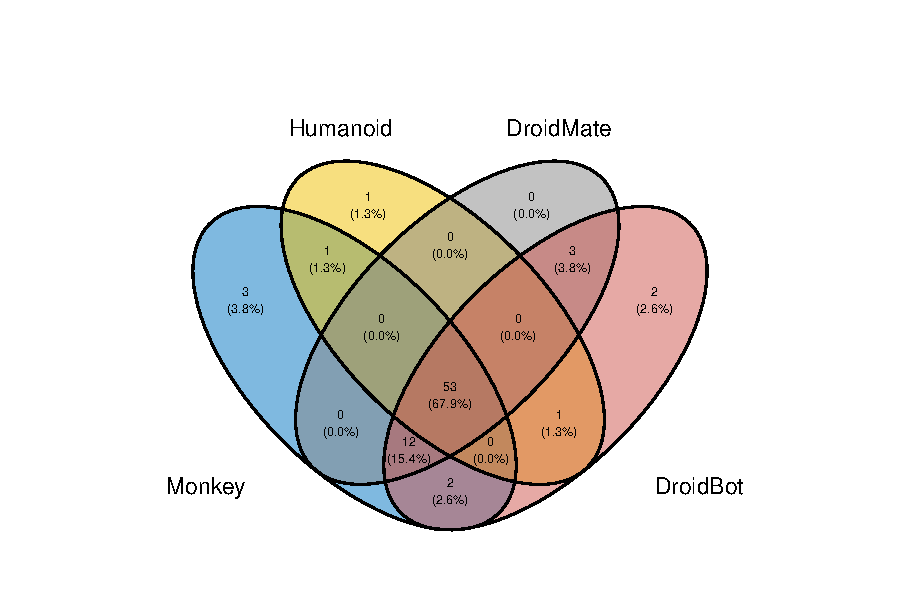
\includegraphics[trim=60 20 0 50,scale=0.9]{images/venn-plot-s1-1.pdf}}
  \caption{Venn Diagram highlighting how the sandboxes from the tools can
    complement each other.}
  \label{fig:venn-plot1}
\end{figure}


Altogether, ignoring the \joke tool, our study reveals that from $58.33$\% (Humanoid)
to $76.04$\% (DroidBot) of the malicious apps investigated in our study can be
detected using the sandboxes generated after running the test case tools with the support of the
DroidFax static analysis algorithms. Besides that, in the first execution (WS), none of the
resulting sandboxes could detect 18 malwares in our dataset ($18.75$\%). According to
the Euphony tool~\cite{hurier2017euphony}, $12$ of these $18$ malwares are \emph{adwares}, $3$ are \emph{trojans}, $2$ are
PUPs (\emph{Potentially Unwanted Program}), and one is an \emph{exploit}. In what follows
we present more details of representative malwares considered
in our dataset.

First, consider the malicious version of the app \texttt{com.andoop.flyracing}---which only the DroidBot and
Humanoid sandboxes were able to detect. 
In this particular case, the malicious version changed the Android Manifest file,
adding permissions to receive and send SMS messages
(Listing~\ref{lst:androidManifest}). With these permissions, malicious apps may get money
fraudulently by sending messages without user confirmation, or may monitor messages or delete
them without showing them to user. 

Moreover, after decompiling this malware, we also observed that the malicious version of the
\texttt{MainService} class introduced a
behavior that collects sensitive information (the International Mobile
Equipment Identity, IMEI) and sends it using an SMS message
(Listing~\ref{lst:mainService}). 

\begin{lstlisting}[caption={Diffs in the \texttt{com.gau.screenguru.finger}
      AndroidManifest file of the malicious
      version}, language=Java,
    basicstyle=\fontsize{8}{6}\selectfont\ttfamily,
    label={lst:androidManifest}]

67:M >    <uses-permission android:name="android.permission.RECEIVE_SMS"/>
68:M >    <uses-permission android:name="android.permission.SEND_SMS"/>
\end{lstlisting}

\begin{lstlisting}[caption={Diffs in the malicious version
      of the class \texttt{com.android.main.MainService}
      (app \texttt{com.gau.screenguru.finger})},
      language=Java, basicstyle=\fontsize{8}{6}\selectfont\ttfamily,
      label={lst:mainService}]

492:M > localObject2 = (TelephonyManager)getSystemService("phone");
493:M > if (localObject2 != null)
494:M > {
495:M >  this.imei = ((TelephonyManager)localObject2).getDeviceId();
496:M >  this.imsi = ((TelephonyManager)localObject2).getSubscriberId();
497:M >  this.iccid = ((TelephonyManager)localObject2).getSimSerialNumber();
498:M > }
// [...]
519:M > if ("".equals(this.destMobile)) {
520:M >  getDestMobile();
521:M > }
522:M > sendSMS(this.destMobile, "imei:" + this.imei)
\end{lstlisting}

The malicious version of the app \texttt{com.happymaau.MathRef} also changes
the manifest file to require additional permissions as well as change
the behavior of the app (with malicious code). All sandboxes were able to
detect this malware.
In this case, the malicious version of the app changed the Android Manifest file,
requiring permissions to access the network and WiFi states (Listing~\ref{lst:androidManifest2}).
These changes allow an app
to view the status of all networks and make changes to configured WiFi-fi networks. 


\begin{lstlisting}[caption={Diffs in the \texttt{com.happymaau.MathRef}
      AndroidManifest file of the malicious
      version}.
      , language=XML,
    basicstyle=\fontsize{8}{6}\selectfont\ttfamily,label={lst:androidManifest2}]

165:M >    <uses-permission android:name="android.permission.ACCESS_NETWORK_STATE"/>
166:M >    <uses-permission android:name="android.permission.ACCESS_WIFI_STATE"/>
\end{lstlisting}


We also observed that the malicious version introduces a method \texttt{a},
that actually collects network and WiFi information, like Mac address and the network state
(see Listing~\ref{lst:d}). This information is then shared using an
HTTP request. 

\begin{lstlisting}[caption={Diffs in the malicious version
      of the class \texttt{com.mn.vymq.b.d}
      (app \texttt{com.happymaau.MathRef})},
      language=Java, basicstyle=\fontsize{8}{6}\selectfont\ttfamily,
      label={lst:d}]

105:M > private String a(Context paramContext)
106:M > {
107:M >	String str = ((TelephonyManager)paramContext.getSystemService("phone")).getDeviceId();
108:M > StringBuilder localStringBuilder = new StringBuilder();
109:M > localStringBuilder.append(str);
110:M > paramContext = (WifiManager)paramContext.getSystemService("wifi");
111:M > if (paramContext == null) {}
112:M >  for (paramContext = null;; paramContext = paramContext.getConnectionInfo())
113:M >  {
114:M >   if (paramContext != null)
115:M >    {
116:M >      paramContext = paramContext.getMacAddress();
117:M >      if (paramContext != null) {
118:M >       localStringBuilder.append(paramContext);
119:M >      }
120:M >    }
121:M >    return a(localStringBuilder.toString());
122:M >  }
123:M > }
\end{lstlisting}


All computed sandboxes also detected the malicious version of the app \texttt{ru.qixi.android.smartrabbits}.
This particular malware also changes the Android Manifest file, requesting permission to access location service (Listing~\ref{lst:androidManifest3}).
This permission allows access location features, such as the Global Positioning System (GPS) on the phone, if it is enabled.
Malicious applications can use these features to determine where the phone owner is, which is a
general privacy threat. 

\begin{lstlisting}[caption={Diffs in the \texttt{com.happymaau.MathRef}
      AndroidManifest file of the malicious
      version}.
      , language=XML,
    basicstyle=\fontsize{8}{6}\selectfont\ttfamily,label={lst:androidManifest3}]

8:M >    <uses-permission android:name="android.permission.ACCESS_COARSE_LOCATION"/>
9:M >    <uses-permission android:name="android.permission.ACCESS_FINE_LOCATION"/>
\end{lstlisting}

In addition, the malicious app clandestinely monitors the geographic location of the user and sink
these information to a web server. Listing~\ref{lst:c} shows how
the method \texttt{c}, from \texttt{q} class, collects these sensitive information. 

\begin{lstlisting}[caption={Diffs in the malicious version
      of the class \texttt{net.crazymedia.iad.d.q}
      (app \texttt{ru.qixi.android.smartrabbits})},
      language=Java, basicstyle=\fontsize{8}{6}\selectfont\ttfamily,
      label={lst:c}]


65:M > private Location c(Context paramContext)
66:M > {
67:M > try
68:M >  {
69:M >  if (Arrays.asList(paramContext.getPackageManager().getPackageInfo
              (paramContext.getPackageName(),4096).requestedPermissions).contains
              ("android.permission.ACCESS_FINE_LOCATION"))

70:M >   {
71:M >    paramContext = (LocationManager)paramContext.getSystemService("location");
72:M >    Criteria localCriteria = new Criteria();
73:M >    localCriteria.setAccuracy(1);
74:M >    localCriteria.setAltitudeRequired(false);
75:M >    localCriteria.setBearingRequired(false);
76:M >    localCriteria.setCostAllowed(true);
77:M >    localCriteria.setPowerRequirement(1);
78:M >    paramContext = paramContext.getLastKnownLocation
                    (paramContext.getBestProvider(localCriteria, true));
                    
79:M >    return paramContext;
80:M >   }
81:M >  }
82:M >  catch (PackageManager.NameNotFoundException paramContext)
83:M >  {
84:M >   paramContext.printStackTrace();
85:M >   return null;
86:M >  }
87:M >  catch (Exception paramContext)
88:M >  {
89:M >   paramContext.printStackTrace();
90:M >  }
91:M >  return null;
92:M > }
\end{lstlisting}


Finally, the \texttt{com.andoop.flyracing} case is among the apps that none sandbox detected the
malicious version. Indeed, the malicious version only changes the Android Manifest file,
modifying the meta-data \texttt{ADMOB\_PUBLISHER\_ID}. Nonetheless, the AdMob is a monetizing
service provided by Google, and changing the AdMob \emph{publisher identifier} account redirects
the advertisement's revenue to another destination. Therefore, it might exist specific
modifications to the Android manifest file that might complement the mining sandbox
approach into the task for detecting malwares. 

\begin{lstlisting}[caption={Diff in the file \texttt{com.andoop.flyracing}
      AndroidManifest file of the malicious version.
      \texttt{B} stands for
      the benign version, while \texttt{M} stands for the malign version.}, language=XML,
    basicstyle=\fontsize{8}{6}\selectfont\ttfamily,label={lst:app65b}]

1:B < <meta-data android:name="ADMOB_\PUBLISHER_\ID"
                     android:value="a14cf7346295891"/>
---
1:M > <meta-data android:name="ADMOB_\PUBLISHER_\ID"
                     android:value="a14f099bfbf3c61"/>
\end{lstlisting}



\subsection{Results of the second study: Using taint analysis to mine Android malwares}\label{sec:res-ss}

In this second study we used a taint analysis approach to mine differences between the
benign and malicious versions of the 96 Android apps in our dataset. To this end we leverage the FlowDroid
%\kn{ Have we cited flowdroid before. If yes, ignore my comment} 
tool, which tracks how sensitive information flows through the apps using taint analysis algorithms.
Regarding accuracy, the taint analysis approach detected $58$ out of the $96$ pairs in our dataset ($60,42$\%). That is,
using the taint analysis implementation of FlowDroid alone outperforms the Monkey, DroidMate,
and Humanoid sandboxes computed in the second execution (without the DroidFax static analysis
algorithms). This result shows that static analysis algorithms are promising for mining
sandboxes, demystifying previous claims in the literature. 

\begin{finding}
  The performance of FlowDroid to identify malicious behavior
  is equivalent to the performance of the
  mining sandbox approach supported by dynamic analysis only---i.e., without
  the DroidFax static analysis algorithms.
\end{finding}

Additionally, we investigate if we could benefit from combining the
static analysis strategies from FlowDroid and DroidFax. Figure~\ref{fig:venn-plot2} shows a
Venn-diagram summarizing the results. So, when combining
the results from FlowDroid and DroidFax, we were able to detect
$67$ of the malicious apps ($69.79$\%), a result compatible
to the performance we found as response to the first execution of the
test case generation tools---which also considers the DroidFax
static analysis algorithms. More interesting, from those $67$
malicious apps identified, $33$ pairs had been found by
both tools (FlowDroid and DroidFax), even though they follow
a completely different static analysis approach. Furthermore,
FlowDroid shows to be more effective than DroidFax alone, detecting $25$ malicious
apps that had not been detected by DroidFax (while DroidFax detected $9$
malicious apps that had not been detected by FlowDroid).

\begin{finding}
  Integrating the results of static analysis tools
  (such as FlowDroid and DroidFax) seems promising,
  leading to a performance similar to that achieved
  when combining test case generation tools with the
  DroidFax static analysis algorithms. 
\end{finding}

\begin{figure}
  \centering{
  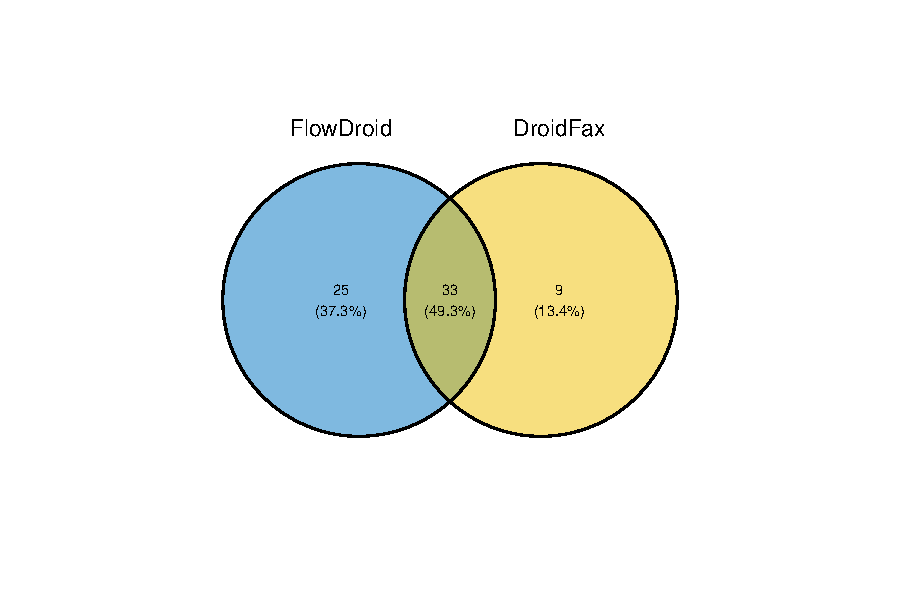
\includegraphics[trim=60 20 0 50,scale=0.7]{images/venn-plot-s2-1.pdf}}
  \caption{Venn Diagram highlighting the possible benefits of
    integrating FlowDroid and DroidFax.}
  \label{fig:venn-plot2}

\end{figure}

The execution of FlowDroid is also feasible: the analysis takes only
32.08 seconds per app on average, totaling a processing time of 52
minutes to analyze all 96 pairs of Android apps.
Even though the time to execute the FlowDroid analysis depends on the size
of the app, the longest run took only 437 seconds. 

Finally, we highlight that FlowDroid was able to detect $4$ malwares among the $18$ malicious Android apps that had not
been detected by the sandboxes constructed in the first study. Among these
four malwares, $2$ are \emph{trojans}, $1$ is an \emph{exploit}, and 1 is an \emph{adware}.

\begin{finding}
  Although FlowDroid presents a performance similar
  to that of using the dynamic analysis approach for mining sandboxes,
  it was able to detect four additional malwares (out of the
  18) that had not been detected in the first study. 
\end{finding}

%% For instance, FlowDroid reveals an additional source-sink path in
%% the \texttt{com.yy.fontmaster} app (see Figure~\ref{fig:sourcesink}. This  a possible malicious behaviors. The Figure \ref{fig:sourcesink}, presents the paths source (blue border) and sink (orange border) from benign and malicious apps.

%% \begin{figure}[ht]%
%%     \centering
%%     \subfloat[\centering Path source/sink from benign app]{{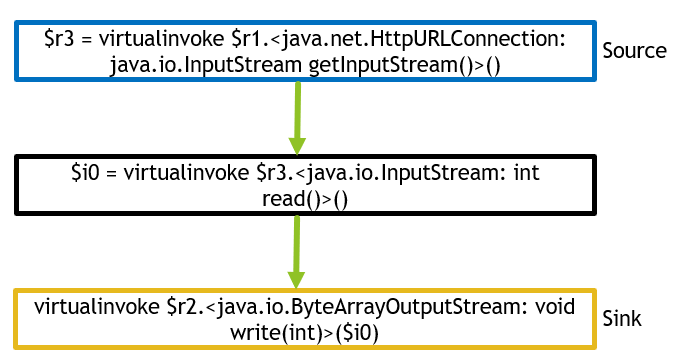
\includegraphics[width=5cm]{images/pathbenign.png} }}%
%%     \qquad
%%     \subfloat[\centering Path source/sink from malicious app]{{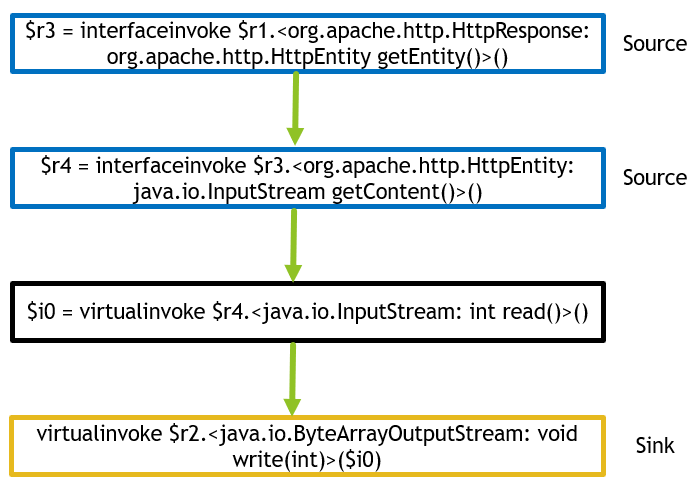
\includegraphics[width=5cm]{images/pathmalicious.png} }}%
%%     \caption{Pairs source/sink different (B/M)}%
%%     \label{fig:sourcesink}%
%% \end{figure}

\subsection{Discussion}\label{sec:discussion}

Our research reinforces the importance of exploring, the contributions of each component used in surveys. The \blls suggested a precision of almost $70\%$ of dynamic analysis tools to differentiate between  the benign and malicious app. However, when our work went into the details of the methodology adopted by \blls, it discovered that in their research, the authors ignore the fact that DroidFax tool statically analyzes the Android apps. Thereby, our research isolates the contribution of each analysis component (static and dynamic), and reveals that in the best case, dynamic analysis tools obtained a performance of $63.54\%$, showing an overestimation of the performance of the dynamic analysis tools for mining sandboxes at \blls.

Besides that, we also found that static analysis, performed by taint analysis algorithms, detected $60,42\%$ malware analyzed.  That fact made evident that it is possible to leverage sandboxes, complementing dynamic analysis tools with taint analysis algorithms. Researchers and apps developers could investigate the use of new static analysis techniques, or a combination of different approaches, to help developers on the task of developing safer apps.

Our results show that static analysis in short had an impact on the \blls and were responsible for improving the results of the tools, between $16.44\%$ and $51.79\%$, which answers our first research question (RQ1). Table \ref{tab:fs} also summarizes our findings addressing the second research question (RQ2). We realized that disregarding the static analysis algorithms, Humanoid had the biggest performance drop, obtaining an effective performance of $28.12\%$. The least affected tool was DroidBot, proving to be the tool with better effective performance in terms of the number of detected malware, obtaining an effective performance of $63.54\%$. Finally, we answered our last research question (RQ3) when we leverage the sandbox, complementing the dynamic analysis with taint analysis algorithms, showing that $69.79\%$-$82.29\%$ of malware can be now uncovered by the static analysis  complement. As a result, the number of malicious apps detected increased in all cases, achieving in the best case, $82.29\%$ with DroidBot , evidencing that a sandbox can be further boosted when coupled with new static analysis techniques. Dynamic analysis coupled with taint analysis algorithms showed a better performance than all five tools explored at \blls, even when they constructed a sandbox by combining all test generation tools when they achieved $75.49\%$ of malware detection. Table \ref{tab:tanted} displays an increase of malware detection on all tools explored in our research.


\begin{table}[ht]
\centering
\begin{tabular}{lccc}\toprule
 Test Generation & FlowDroid & Total & \%\\
 Tool & Increase  &  & \\ \midrule
 DroidBot & 6 & 79 & 82.29\\
 Monkey & 7 &  78 & 81.25 \\
 DroidMate & 7 & 75 & 78.12  \\
 Humanoid & 16 & 72 & 75.00 \\
 Joker & 25 & 67 & 69.79  \\\midrule
 
\end{tabular} 
\caption{Malwares detected in 96 pair (B/M) increased by Taint analysis Algorithms}
\label{tab:tanted}
\end{table}


%%here we also have to write about the intersection between droidfax and tainted analysis now, and about what 1 reveled and other dont, and otherwise. 


%Here we can write about MOTIVATION EXAMPLES.
